% Options for packages loaded elsewhere
\PassOptionsToPackage{unicode}{hyperref}
\PassOptionsToPackage{hyphens}{url}
%
\documentclass[
]{book}
\usepackage{lmodern}
\usepackage{amsmath}
\usepackage{ifxetex,ifluatex}
\ifnum 0\ifxetex 1\fi\ifluatex 1\fi=0 % if pdftex
  \usepackage[T1]{fontenc}
  \usepackage[utf8]{inputenc}
  \usepackage{textcomp} % provide euro and other symbols
  \usepackage{amssymb}
\else % if luatex or xetex
  \usepackage{unicode-math}
  \defaultfontfeatures{Scale=MatchLowercase}
  \defaultfontfeatures[\rmfamily]{Ligatures=TeX,Scale=1}
\fi
% Use upquote if available, for straight quotes in verbatim environments
\IfFileExists{upquote.sty}{\usepackage{upquote}}{}
\IfFileExists{microtype.sty}{% use microtype if available
  \usepackage[]{microtype}
  \UseMicrotypeSet[protrusion]{basicmath} % disable protrusion for tt fonts
}{}
\makeatletter
\@ifundefined{KOMAClassName}{% if non-KOMA class
  \IfFileExists{parskip.sty}{%
    \usepackage{parskip}
  }{% else
    \setlength{\parindent}{0pt}
    \setlength{\parskip}{6pt plus 2pt minus 1pt}}
}{% if KOMA class
  \KOMAoptions{parskip=half}}
\makeatother
\usepackage{xcolor}
\IfFileExists{xurl.sty}{\usepackage{xurl}}{} % add URL line breaks if available
\IfFileExists{bookmark.sty}{\usepackage{bookmark}}{\usepackage{hyperref}}
\hypersetup{
  pdftitle={Transparencia y Reproducibilidad en Investigación Social},
  pdfauthor={Julio Iturra y Martín Venegas},
  hidelinks,
  pdfcreator={LaTeX via pandoc}}
\urlstyle{same} % disable monospaced font for URLs
\usepackage{longtable,booktabs}
% Correct order of tables after \paragraph or \subparagraph
\usepackage{etoolbox}
\makeatletter
\patchcmd\longtable{\par}{\if@noskipsec\mbox{}\fi\par}{}{}
\makeatother
% Allow footnotes in longtable head/foot
\IfFileExists{footnotehyper.sty}{\usepackage{footnotehyper}}{\usepackage{footnote}}
\makesavenoteenv{longtable}
\usepackage{graphicx}
\makeatletter
\def\maxwidth{\ifdim\Gin@nat@width>\linewidth\linewidth\else\Gin@nat@width\fi}
\def\maxheight{\ifdim\Gin@nat@height>\textheight\textheight\else\Gin@nat@height\fi}
\makeatother
% Scale images if necessary, so that they will not overflow the page
% margins by default, and it is still possible to overwrite the defaults
% using explicit options in \includegraphics[width, height, ...]{}
\setkeys{Gin}{width=\maxwidth,height=\maxheight,keepaspectratio}
% Set default figure placement to htbp
\makeatletter
\def\fps@figure{htbp}
\makeatother
\setlength{\emergencystretch}{3em} % prevent overfull lines
\providecommand{\tightlist}{%
  \setlength{\itemsep}{0pt}\setlength{\parskip}{0pt}}
\setcounter{secnumdepth}{5}
\usepackage{booktabs}
\ifluatex
  \usepackage{selnolig}  % disable illegal ligatures
\fi
\usepackage[]{natbib}
\bibliographystyle{apalike}

\title{Transparencia y Reproducibilidad en Investigación Social}
\author{Julio Iturra y Martín Venegas}
\date{2021-07-02}

\begin{document}
\maketitle

{
\setcounter{tocdepth}{1}
\tableofcontents
}
\hypertarget{intro}{%
\chapter{Introducción}\label{intro}}

Imagine que usted es un chef, y como tal, disfruta enormemente del arte de cocinar. Como amante de la cocina, cada vez que alguna celebración especial se avecina, es tradición preparar sus mejores recetas para sus invitados. Sin embargo, en esta ocasión, la celebración se llevará a cabo en un restaurante, lo cual implica que la preparación de la comida no depende de usted. Con bastantes dudas, usted accede, teniendo en mente la siguiente pregunta: ¿Cómo puedo tener certeza de que se seguirán los procedimientos adecuados para que la preparación sea de calidad? Pues, estimado lector, es esta la pregunta que subyace a todo el proceso que engloba al conocimiento científico.

La ciencia, al igual que la cocina, no se trata solamente de los productos. Una preparación no aparece por generación espontánea, sino que requiere el seguimiento riguroso de una receta, en la cual usamos los ingredientes adecuados, la cantidad apropiada y los tiempos de cocción. Esta receta no solo contribuye a la preparación de la comida, sino que hace posible que dicho plato pueda ser \textbf{reproducido} cada vez que se lo desee, garantizando el mismo resultado. Entonces, como buen chef, la respuesta a la pregunta no es tan compleja: necesitamos ser capaces de evaluar el proceso de elaboración de la comida para asegurarnos de que es el adecuado. Dicho de otro modo, el proceso de preparación debe ser \textbf{transparente} y estar abierto al escrutinio de otros cocineros expertos, como también para quienes estén adentrándose en la cocina. En el caso de la comida, que el restaurante cuente con una cocina abierta o construida en torno a ventanales bastaría para lograr este objetivo. Sin embargo, dentro del campo de la ciencia ¿cómo logramos que el proceso de producción del conocimiento científico esté abierto al escrutinio público?

Esta pregunta puede ser algo engañosa ¿acaso los procesos de investigación en la ciencia no están ya abiertos al escrutinio público? La narrativa actual pareciese sugerir que no. En el último tiempo ha primado el diagnostico de que la ciencia está viviendo una crisis, donde polémicas situaciones de malas prácticas académicas han salido a la luz. Un ejemplo de estas malas prácticas es el falseamiento de datos. Uno de los casos más emblemáticos es el de Diderik Stapel, una figura académica con alto prestigio en el campo de la psicología social a quién se le acusó y confirmó de falseamiento de datos. Más de 10 años de investigación y 150 artículos -algunos de ellos en las revistas más prestigiosas- fueron puestos en duda a raíz de las malas prácticas de Stapel. Así también el trabajo de muchos colegas y estudiantes fue desacreditado. El caso del ex doctor Stapel acabó en la revocación de su doctorado, la retracción de 58 artículos de investigación y, prácticamente, el fin de su carrera académica.

Casos como el de Diderik Stapel existen muchos \citep[ver][]{abrilruiz_Manzanas_2019}, sin embargo, no son las prácticas más recurrentes. Dentro de la investigación científica existen una serie de prácticas que caen en un terreno gris cuando se trata de su evaluación ética, estas son las llamadas \emph{prácticas cuestionables de investigación}. La preocupación dentro de la comunidad científica es que la acumulación y la poca fiscalización de estas prácticas lleven a una ciencia poco transparente, con dificultad en torno a la reproducibilidad de los análisis y de sus resultados, y que a la larga se pierda la confianza en el quehacer científico.

La perdida de la confianza en el quehacer científico afecta el objetivo de las ciencias sociales. Generalmente se tiene la concepción de que es parte de las tareas de los científicos sociales el contribuir al bienestar de la sociedad por la vía de las herramientas de investigación. Esta es la noción de las ciencias sociales como un bien público \citep{thibodeaux_Production_2016}. Bajo esa idea, los efectos de una crisis de credibilidad tienen dos posibles efectos concretos en las ciencias sociales. Primero, la falta de credibilidad podría afectar la confianza en los hallazgos y en las disciplinas que componen las ciencias sociales. Ya existe evidencia sobre un incremento de desconfianza hacia los científicos en países como Estados Unidos \citep{motta_Dynamics_2018} y sumarle una crisis de la ciencia a esa situación solo generaría un ambiente mucho más complejo. Segundo, y estrechamente relacionado a lo anterior, una perdida de credibilidad en la ciencia podría impactar en la elaboración de políticas sociales, mal orientando las prioridades y los recursos del país. Si se quieren evitar estas situaciones, es necesario tomar cartas en el asunto y orientar los esfuerzos a devolverle la credibilidad a las ciencias sociales.

Este manual busca contribuir a una ciencia social más creíble, basándose en el marco de la ciencia abierta. La ciencia abierta se entiende como:

\begin{quote}
``\ldots la práctica de la ciencia de manera que otros puedan colaborar y contribuir, donde los datos de la investigación, las notas de laboratorio y otros procesos de investigación estén disponibles libremente, en términos que permitan la reutilización, redistribución y reproducción de la investigación y sus datos y métodos subyacentes''. (FORSTER, Open Science Teaching Resource)
\end{quote}

Dentro de la ciencia abierta, nos centraremos en dos conceptos: transparencia y reproducibilidad. Si seguimos la metáfora de la cocina que planteamos en un principio, la transparencia y la reproducibilidad son dos conceptos similares, pero no idénticos. La transparencia implicaría la posibilidad de evaluar y poner en discusión la receta y la ejecución de la misma. En cambio, la reproducibilidad apuntaría a que la receta sea lo suficientemente clara y precisa para que el mismo plato, con el mismo sabor, pueda ser preparado por cualquier persona que contase con los ingredientes y recursos necesarios. En el campo de las ciencias, esta distinción la hacemos entre: 1) la transparencia de los procesos de producción científica (e.g.~transparentar el plan de análisis) y 2) la reproducibilidad de los análisis en los artículos (e.g.~código de procesamiento y análisis de datos permite reproducir el artículo). Este manual estará estructurado en torno a estas dos conceptos.

Relacionado al primer concepto (transparencia), haremos un barrido un tanto más detallado sobre la crisis de la reproducibilidad que aquí hemos mencionado brevemente. Ahondaremos en los factores que contribuyen a su reproducción, a las razones éticas por el cuales es necesario hacer un cambio y en las recomendaciones que se pueden seguir para adoptar ciertos principios de transparencia. En el caso del segundo concepto (reproducibilidad), nos centraremos en los análisis reproducibles, teniendo un carácter mucho más práctico. Presentaremos las distintas consideraciones que hay que tener para que un análisis sea fácilmente reproducible, desde tipos de flujos de trabajo hasta herramientas específicas que faciliten la reproducibilidad de los análisis.

Estimado investigador o investigadora de las ciencias sociales, este documento va dirigido a usted. Independiente de su disciplina, de su trayectoria académica o de su conocimiento previo con respecto a estas temáticas, en este manual tenemos dos simples objetivos. El primero es que usted pueda convencerse de que, efectivamente, es necesario dar un giro en la forma que hacemos ciencia actualmente y que la adopción de prácticas relacionadas a la ciencia abierta son el primer paso en ese giro. El segundo es poder instruirlo en esa adopción de prácticas, particularmente en lo que respecta a la transparencia y reproducibilidad. Al final de este manual, usted será capaz tanto de argumentar por qué la transparencia y la reproducibilidad son un paso importante en el avance de las ciencia sociales, así como también contará con una serie de herramientas para llevar esto al quehacer académico del día a día.

\hypertarget{transparencia}{%
\chapter{Transparencia}\label{transparencia}}

Esta sección tratará sobre la transaprencia en la investigación cientifica, haciendo enfásis en las ciencias sociales. Nuestro objetivo es poder comunicar de forma clara y concisa tres puntos: a) qué es la transparencia, b) por qué la necesitamos y c) cómo podemos adoptarla. En esta sección verenmos los dos primeros puntos, luego, en la sección de herramientas presentaremos algunas formas de adoptar la transparencia. La tónica de este escrito es la práctica, es decir; todo lo que presentemos acá tiene la finalidad de servir de camino para poder aprender y aprehender herramientas que promueven la transparencia. Dicho esto, comenzemos con los dos primeros puntos.

\hypertarget{quuxe9-es-la-transparencia-un-concepto-multidimensional}{%
\section{¿Qué es la transparencia? Un concepto multidimensional}\label{quuxe9-es-la-transparencia-un-concepto-multidimensional}}

Nuestro punto de partida es que la transparencia es un concepto amplio y multidimensional. Por eso, antes de adentrarnos en su complejidad, comenzemos con una definición de diccionario para comprender lo más básico en la idea de transparencia. Según la Real Academia Española la transparencia es la cualidad de un cuerpo que permite ver a travez de él. Un gran ejemplo para llevar esta definición a la práctica es el vidrio de una ventana. La transparencia del vidrio nos permite ver con claridad lo que está el otro lado, como por ejemplo un paisaje. Sin embargo, ¿qué ocurre cuándo la transparencia del vidrio se va perdiendo? La respuesta es simple, pero potente: la claridad con la que veíamos el paisaje se va difuminando. Esta perdida de claridad puede dar como resultado que nuestra observación del paisaje se torne ambigua y erronea, o dicho de otro modo, cada vez será más dificil analizar el paisaje. En esta metafora, el paisaje sería equivalen al proceso de producción cientifica, y el vidrio representa la claridad con la que podemos analizar estos procesos. De esta manera, la base de la idea de transparencia es que permite analizar con claridad un fenomeno, una situación, o en este caso, un proceso.

¿Qué implica un proceso cientifico transparente? Ya existen algunas respuestas a esta pregunta. Por ejemplo, \citet{breznau_Does_2021} entiende la transparencia como una forma en que los investigadores pueden revelar el proceso, ideas y materiales que sustentan un argumento o una teoría, con tal de contribuir a una comunidad científica más ética. Otra perspectiva es la de \citet{aczel_consensusbased_2020}, quienes proponen a la transparencia como un principio que permite evaluar y reproducir los hallazgos científicos, así como también a sintetizar investigaciones y contribuir a la ejecución de metanálisis. Estas perspectivas son una primera aproximación a las implicancias de un proceso cientifico transparente, no obstante, no son una presentación exhaustiva del concepto.

Para abarcar la complejidad del concepto de transparencia, y las múltuiples formas que puede adoptar, nos basamos en la taxonomía de \citet{elliott_Taxonomy_2020}. La taxonomía se basa en cuatro grandes preguntas: ¿por qué?, ¿quienes? ¿qué? y ¿cómo? Cada una de estas preguntas tiene al menos una dimensión asociada. La primera pregunta se refiere a los propósitos por los cuales adoptar la transparencia; la segunda pregunta apunta a la audiencia que está recibiendo la información; la tercera pregunta hace alusión al contenido qué es transparentado y la cuarta pregunta consiste en cuatro dimensiones distintas sobre cómo adoptar la transparencia: actores, mecanismos, tiempo y lugar. También, la taxonmía propone una dimensión sobre los peligros que podrían afectar a las iniciativas que busquen promover la transparencia. Aunque esta última dimensión no es una forma de transparencia -en el mismo sentido que las otras dimensiones-, si tiene relevancia en tanto permite mejorar las iniciativas de transparencia. Una representación gráfica puede verse en la Figura N° \ref{fig:taxonomy}.

\begin{figure}

{\centering 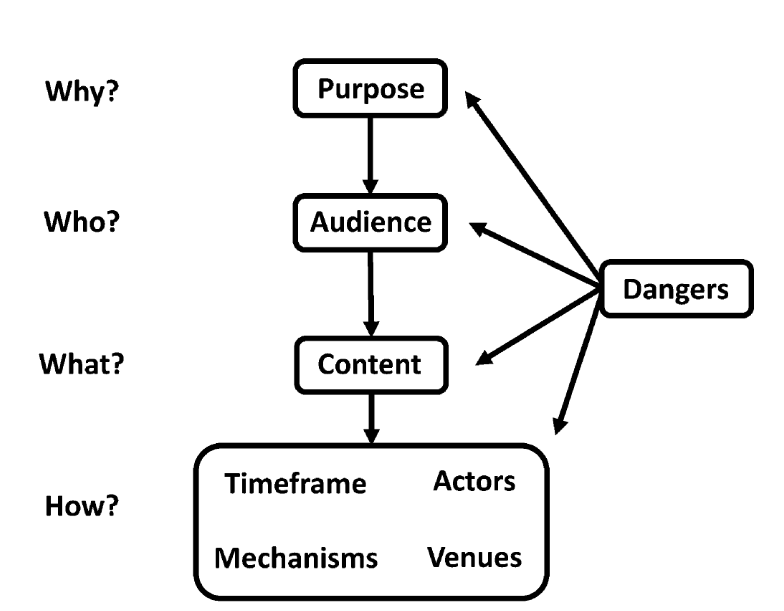
\includegraphics[width=1\linewidth]{docs/images/taxonomy} 

}

\caption{Taxonomía de Transparencia}\label{fig:taxonomy}
\end{figure}

Para comprender mejor la taxonomía la Figura N° \ref{fig:tabtax} presenta una versión detallada de cada dimensión en conjunto a una lista no exhaustiva de variaciones. Por ejemplo, la dimensión del propósito sintetiza varios de los puntos que ya se han señalado en la literatura sobre ciencia abierta: hacer la ciencia más replicable, facilitar la interacción crítica, facilitar el reanalisis de resultados, entre otros. La mayoría de estos propositos están estrechamente relacionados con el horizonte de una ciencia con mayor credibilidad. Dentro de las dimensiones restantes, existe una en particular que queremos recalcar: los contenidos. Aquí, los distintos contenidos que pueden ser transparentados van desde cosas complejas como los juicios de valor, hasta lo más concreto como datos, métodos y materiales, o dicho de otra forma, el diseño de investigación. El diseño de investigación es uno de los que más se ha promovido la transparencia últimamente, especialmente a raíz de los pre-registros. Profundizaremos en esto más adelante en el escrito.

En síntesis, un proceso de investigación transparente es uno que se puede evaluar con claridad y facilidad. La taxonomía de \citet{elliott_Taxonomy_2020} nos ayuda a comprender las diversidad dimensiones en las que se puede pensar la idea de transparencia. Sin embargo, aun existe la pregunta del \emph{por qué}. ¿Por qué es relevante la idea de transparencia? La dimensión de propositos de la taxonomía ya nos ha dado algunas pistas: la ciencia puede ser mejor. Y no solo eso, sino que inclusive podria estar en crisis.

\begin{figure}

{\centering 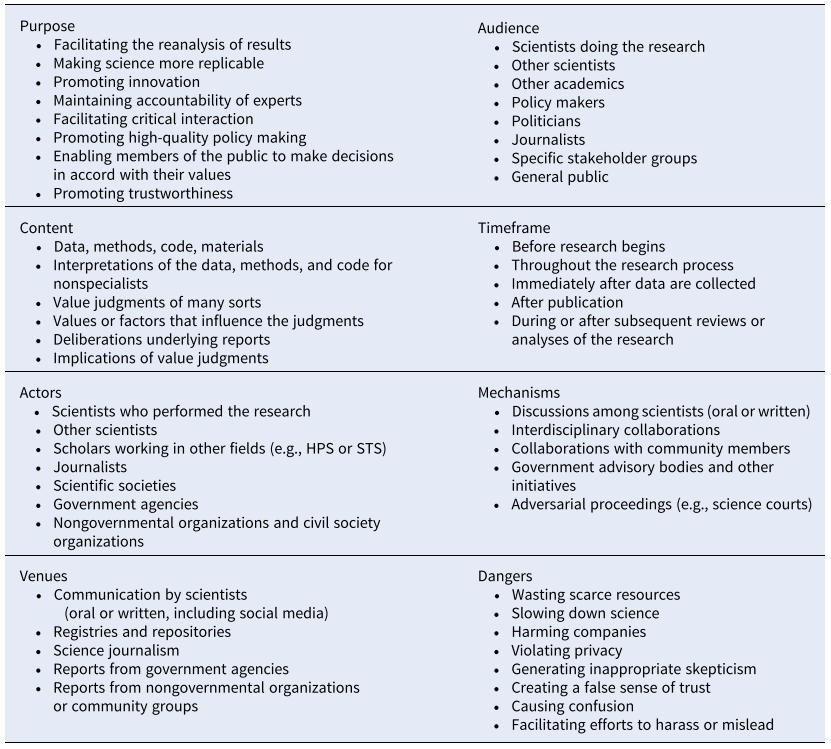
\includegraphics[width=1\linewidth]{docs/images/table_tax} 

}

\caption{Variaciones por dimensión de transparencia}\label{fig:tabtax}
\end{figure}

\hypertarget{crisis-en-las-ciencias}{%
\section{¿Crisis en las ciencias?}\label{crisis-en-las-ciencias}}

En los últimos años, ha venido tomando fuerza la idea de que existe una crisis en la ciencia. Esta idea se basa en el diagnóstico de que gran parte de los artículos cientificos en distintas discplinas no son posibles de reproducir ni replicar. Tanto la reproducibilidad (emplear el mismo diseño y datos para reproducir los hallazgos de un artículo) o la replicabilidad (emplear el mismo diseño y distintos datos para obtener los mismos resultados) son componentes centrales de la ciencia. Es más, algunos de los mecanismos que permiten el avance del conocimiento cientifico son el escrutinio y la verificabilidad de sus hallazgos, por lo que un fallo en el cumplimiento de estos es un golpe directo a la credibilidad de la ciencia. La pregunta es ¿existe realmente una crisis en las ciencias?

Unas de las fuentes más comunmente citadas para introducir la idea de crisis es una encuesta realizada en la revista \emph{Nature}. En esta encuesta, \citet{baker_500_2016} logró obtener las opiniones de poco más de 1,500 investigadores de discplinas como la quimica, ingenerías y la medicina, sobre tópicos relacionados a la reproducibilidad en las ciencias. El resultado principal muestra que un \textbf{90\% de los encuestados está de acuerdo en la existencia una crisis}, donde un 52\% piensa que es una gran crisis y un 38\% la percibe como una ligera crisis. En este mismo estudio, se les pregunta por los factores que contribuyen a esta crisis, donde la cultura del \emph{pública o perece} y el \emph{reporte selectivo de resultados} aparecen como los protagonistas. Si bien la encuesta no es una muestra representativa de toda la comunidad cientifica, presenta una panoramica que lleva a, por lo menos, considerar la crisis de la ciencia como tema que merece atención.

Actualmente, existe un cuerpo de literatura que se ha dedicado diagnosticar y proponer alternativas de solución ante la idea de una ciencia en crisis. Dentro del diagnóstico, variados estudios han orientado sus esfuerzos a esclarecer cuáles son los factores que podrían estar influenciando esta crisis. En esta sección, presentaremos estos factores en dos grandes dimensiones. La primera dimensión se relaciona a las prácticas de investigación, especificamente aquellas prácticas que ya sea en menor o mayor grado afectan la credibilidad de los hallazgos cientificos en su conjunto. La segunda dimensión se centrará más en factores institucionales y que no dependen estrictamente de los investigadores. Una vez explicados estos factores, analizeremos como ciertas herramientas que promueven la transparencia en la investigación podrían c

Comenzemos con las prácticas de investigación. Para esquematizar de mejor manera qué es lo problemático de ciertas prácticas, es que utilizaremos el esquema conceptual de \citet{steneck_Fostering_2006}. El esquema parte de una distinción básica entre la \emph{ética en investigación} y la \emph{integridad en investigación}, englobando ambas bajo el gran concepto de \emph{Conducta Responsable de Investigación (RCR)} (ver Figura N° \ref{fig:rcr}. A grandes rasgos, la RCR se puede entender como el ``llevar a cabo la investigación de forma que se cumplan las responsabilidades profesionales de los investigadores, tal y como las definen sus organizaciones profesionales, las instituciones para las que trabajan y, en su caso, el gobierno y el público'' \citep{steneck_Fostering_2006}\footnote{A raíz de esta definición, y también en base al código de conducta detallado por XX es que \citet{abrilruiz_Manzanas_2019} proponen a la siguiente definición: ``la RCR es el conjunto de normas, habitualmente plasmadas en códigos de conducta, que pretenden ser una guía para que nuestras acciones se mantengan dentro de la integridad investigadora'' (p.144).}.

\textbackslash begin\{figure\}

\{\centering 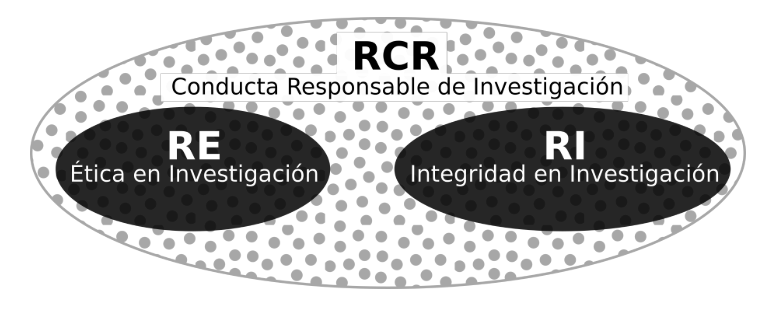
\includegraphics[width=1\linewidth]{docs/images/rcr}

\}

\textbackslash caption\{Conducta Responsable de Investigación. Imagen de \citet{abrilruiz_Manzanas_2019} basada en \citet{steneck_Fostering_2006}\}\label{fig:rcr}
\textbackslash end\{figure\}

Dentro de este concepto, la ética de investigación está relacionada al comportamiento académico visto desde la óptica de los principios morales \citep{steneck_Fostering_2006}, lo que se expresa en tópicos como el uso de datos, los consentimientos informados, el trato con pacientes -en el caso de las ciencias biomedicas-, por dar algunos ejemplos. La definición que ofrece \citet{steneck_Fostering_2006} señala que la ética de investigación se define como ``el estudio crítico de los problemas morales asociados o que surgen en el curso de la investigación'' (p.56) En cámbio, la integridad en investiación se entiende como ``poseer y adherirse firmemente a las normas profesionales, tal y como las señalan las organizaciones profesionales, las instituciones de investigación y, en su caso, el gobierno y el público'' \citep[p.56]{steneck_Fostering_2006}. A diferencia de la ética de investigación, el concepto de identidad está regido por los estándares profesionales más que por los principios morales, su función es plantear una guía clara para la conducta inevestigativa, de ahí que sea el concepto utilizado por distintos códigos de conducta{[}{]}.

\textbackslash begin\{figure\}

\{\centering 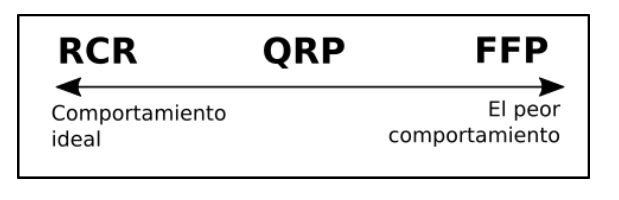
\includegraphics[width=1\linewidth]{docs/images/grad}

\}

\textbackslash caption\{Gradación del comportamiento integro en investigación. Imagen de \citet{abrilruiz_Manzanas_2019} basada en \citet{steneck_Fostering_2006}\}\label{fig:grad}
\textbackslash end\{figure\}
Habiendonos situando dentro del concepto de integridad en la investigación, podemos pasar a delinear las principales prácticas que atentan contra él y que se han propuesto como factores que contribuyen a la crisis en la ciencia. Tanto \citet{steneck_Fostering_2006} como distintos códigos de conducta de universidades e instituciones de financiamiento {[}{]} evalúan las prácticas de investigación en un continuo, que representa cuánto adhieren los investigadores a los principios de integridad cientifica. La Figura N° \ref{fig:grad} esquematiza esta idea mostrando dos extremos, donde a la izquierda está el mejor comportamiento (RCR), y a la derechaa el peor comportamiento (FFP). Las FPP son un abreviación en lengua inglésa para referirse a \emph{Fabrication, Falsification, Plagiarism} (Invención, Falsificación y Plagio), también conocidas como \emph{mala conducta académica}-. En el medio del continuo están las \emph{prácticas cuestionables de investigación} (QRP, por sus siglas en inglés) las cuáles refieren a ``acciones que violan los valores tradicionales de la empresa de investigación y que pueden ser perjudiciales para el proceso de investigación'' \citep[\emph{National Academies of Science} 1992 en][p.58]{steneck_Fostering_2006}. A diferencia de las FFP, las QRP son prácticas que tienen el potencial de dañar la ciencia y no que la dañan directamente (como las FFP).

Comprendidos ambos conceptos, veamos las situaciones que podrían categorizarse como FFP y las que podrían concebirse como QRP.

\hypertarget{mala-conducta-acaduxe9mica-ffp}{%
\subsection{Mala conducta académica (FFP)}\label{mala-conducta-acaduxe9mica-ffp}}

La mala conducta académica suelen ser situaciones polémicas y que muchas veces alcanzan gran conbertura mediatica. El libro de \citet{abrilruiz_Manzanas_2019} presenta una serie de situaciones, en distintas discplinas y años, en las que investigadores han sido descubiertos cometiendo prácticas que atentan directamente a la ciencia. Las situaciones son variadas, existen casos de manipulación de imagenes {[}{]}, exageración de lo registros de laboratorio, o de plano la invención de conjuntos de datos enteros. En esta sección veremos el caso de Diderik Stapel como ejemplo de malas prácticas de investigación y plantearemos la relación que tiene con la transparencia en la investigación.

\hypertarget{diderik-stapel}{%
\subsubsection{Diderik Stapel}\label{diderik-stapel}}

Probablemente, el caso de Diderik Stapel sea uno de los más emblématicos y representativos de este problema. Diderik Stapel era un investigador de la \emph{Tilburg University} que se dedicaba al campo de la psicologóa social. Su carrera se caracterizó por una trayectoria ejemplar, obtuvo su M.A en psicolgía y comunicaciones el año 1991, se doctoró en psicología social el año 1997 y trabajó como profesor asociado primero en la \emph{University of Gronigen} (2000-2006) y dede el 2006 en la Tilburg University. Fue fundador del \emph{Tilburg Institute for Behavioral Economics Research}, del cuál el 2010 se convirtió en decano. Así también, fue galardonado con el premio a la trayectoria académica por la \emph{Social of Experimental Social Psychology}. En breve, Stapel era una figura de alto estatus en el mundo académico, entre 1995 y 2015 publicó aproximadamente 150 artículos en revistas cientificas, algunas de las más prestigiosas (e.g.~\emph{Science}). Sin embargo, el año 2011 se confirmó que gran parte de su trayectoria académica era una farsa.

Después de la verificación de su culpa ante acusaciones de malas prácticas, la carrera de Diderik Stapel acabó. Fue desvinculado de la Tilburg University, se le rebocó su título de doctorado y toda su trayectoria académica fue investigada acusiociamente. El informe final de la investigación encontró que más de 50 de sus artículos eran fraudulentos. De hecho, Stapel ocupa el tercer lugar en \emph{Retraction Watch}, con 58 de sus artículos retractados. A efectos de este escrito, lo que más destacable es que Stapel cometió conductas de mala conducta académica durante más de 15 años. La pregunta es ¿cómo fue esto posible? ¿cómo ninguno de sus colegas, alumnos o co-autores se dio cuenta de sus malas prácticas? La respuesta breve es por la falta de transparencia durante el proceso de investigación.

Los artículos periodisticos que han profundizado en el caso \citep[e.g.][]{carey_Fraud_2011} han relatado parte del proceso investigativo de Stapel. Dentro de los procesos de producción y análisis de datos, Stapel se caracterizaba por hacer todo el trabajo solo y ``a puertas cerradas''. Es decir, nadie más que él tenía acceso a los datos brutos, ni támpoco a la ejecución de las pruebas estadísticas. Generalmente, Stapel compartía con sus colegas y alumnos de doctorado la base de datos lista, con las pruebas estadísticas ya hechas y, claro está, con resultados significativos. Estas prácticas no causaron sospechas durante muchos años, es más, a muchos de sus estudiantes les parecía una práctica normal y eficiente. Además, con el estatus de Stapel ¿qué podría estar mal? Sin embargo, era a raíz de esta práctica que Stapel tenía la oportunidad de inventar y falsificar datos a su conveniencia. Esto explica en gran parte de su trayectoría académica llena de grandes hallazgos.

El caso de Stapel deja un punto base sobre la mesa: la falta de transparencia en el proceso investigativo dio cabida a la mala conducta académica. Cómo nadie más colaboraba con el procesamiento de datos, ni támpoco parecía extraño que asi fuera, las oportunidades para la falsificación de los datos estaba abierta. Ahora, esta no es necesariamente una relación de causalidad, la falta de transparencia no tiene porque terminar en conductas como fabricación o falsificación de datos. Sin embargo, tal y como lo argumentan \citep{oboyle_Chrysalis_2017} si son una oportunidad para violaciones a la integridad cientifíca más sutiles, tales como las QRP.

\hypertarget{pruxe1cticas-cuestionables-de-investigaciuxf3n-qrp}{%
\subsection{Prácticas cuestionables de investigación (QRP)}\label{pruxe1cticas-cuestionables-de-investigaciuxf3n-qrp}}

Recordemos, las QRP son prácticas que en si mismas no dañan directamente la empresa cientifica, pero si tienen el potencial de hacerlo. En la literatura sobre el tema, existen una multiplicidad de términos y listas de prácticas especificas que pueden categorizarse como cuestionables. \citet{abrilruiz_Manzanas_2019} hace una recopilación y traducción de distintos códigos de conducta de distintas universidades y organismos, el cuál nosotros sistematizamos en la Figura N° X. La figura muestra un conjunto de prácticas divididos en cuatro categorías, de acuerdo a si las prácticas tienen que ver con: la redacción y el reporte de los resultados, el procesamiento de los datos, temas de citación y uso de ideas ajenas y, por último, sobre relaciones con otros actores en el campo de la ciencia. El objetivo de esta recopilación es meramente esquemático, en el sentido de poder gatillar la reflexión respecto a la experiencia del lector a partir de algunas situaciones concretas que podráin afectar las investigaciones.

Han habido algunos estudios que han intentado medir directamente la existencia de estas prácticas a través de encuestas cuantitativas. \citet{fanelli_How_2009} hizo un metanálisis que tenía por objetivo sistematizar los resultados de estudios que hasta esa fecha habían abordado las prácticas de investigación desde encuestas cuantitativas. Los resultados mostraron que un 1.97\% de investigadores había inventado datos al menos una vez y que un 33.7\% había realizado alguna vez una QRP como ``borrar puntos de los datos basados en un sentimiento visceral''. Un estudio más reciente, también basado en encuestas cuantitativas sobre prácticas, es el de \citet{john_Measuring_2012}. En este estudio, los resultados mostraron que un 36.6\% de quienes participaron alguna vez habían práctiado alguna QRP. En detalle, analizando los porcentajes práctica a práctica se halló que el 50\% de los psicologos encuestados alguna vez reportaron selectivamente estudios que apoyaran su hipotesis; un 35\% alguna vez reportaron resultados inesperados como esperados; y un 2\% alguna vez reportó datos falsos. Estos estudios son una primera aproximación a la existencia de las QRP en la ciencia.

Existen ciertas prácticas que han sido tratadas con más enfásis en la literatura, y que son las que queremos destacar acá. Por un lado, está el \emph{sesgo de publicación}. A grandes rasgos, los sesgos de publicación se refieren a la publicación exclusiva de resultados significativos, en desmedro de los no significativos. Dicho de otra forma, cuándo el criterio de selección para la publicación de resultados es la significancia, el cuerpo de literatura de esa temática particular comienza a sesgarse. El estudio de \citet{franco_Publication_2014} tiene por objetivo cuantificar esta situación, especificamente en ciencias sociales. En su estudio encontraron un patrón interesante: ``estudios donde la hipotesis principales arrojan resultados nulos son 40\% menos probables de ser publicados en una revista cientifica, en contraste a estudios que arrojen resultados significativos'' \citep[p.41]{christensen_Transparent_2019}. Los descriptivos se pueden ver en la Figura N° \ref{fig:written}.

Otra práctica es la del \emph{p-hacking}\ldots{}

Por último, está el \emph{HARKing}, el cual\ldots{}

Un estudio que se aleja de la encuesta directa sobre prácticas, pero que contribuye estimando cuál es el potencial de que una QRP afecte los resultados de un artículo es el de \citet{simmons_FalsePositive_2011}. En detalle, los autores buscan calcular el \emph{likelihood} de obtener un falso positivo (error Tipo I) de acuerdo a al nivel de manipulación intencionada de los datos. El procedimiento consistió en calcular 15.000 muestras de 20 observaciones por condición de tratamiento para un experimento hipotetico y determinaron cuatro posibles ajustes a los datos: 1) plantear dos variables dependientes correlacionadas, 2) incrementar la muestra entre 20 y 30 casos según condición de tratamiento, 3) controlar por una variable sociodemográfica (género) o plantear una interacción genero y condición de tratamiento y 4) flexibilidad en eliminar alguna condición de tratamiento. Como se puede ver en la Figura N° \ref{fig:fp}, el resultado principal es que a medida que aumenta la cantidad de manipulación en los datos, el likelihood de obtener un falso positivo aumenta progresivamente. Una situación en donde se realicen los cuatro ajustes planteados tiene un 60.7\% de likelihood de encontrar un falso positivo.

Una herramienta que se ha utilizado para estimar la existencia de p-hacking en los cuerpos de literatura es la \emph{p-curve}. La p-curve ``describe la densidad de los \emph{p-values} reportados en una literatura, aprovechando el hecho de que si la hipótesis nula fuera verdadera (es decir, sin efecto), los p-values deben distribuirse uniformemente entre 0 y 1'' \citep[p.67.]{christensen_Transparent_2019}. De esta manera, en cuerpos de literatura que no sufran de p-hacking, la distribución de p-values debería ser asimetrica a la derecha, en cambio, si existe sesgo por p-hacking la distribución de p-values estaría distribuida de forma asimetrica a la izquierda. \citet{simonsohn_Pcurve_2014} proponen esta herramienta y la prueban en dos muestras de artículos de la \emph{Journal of Personality and Social Psychology (JPSP)}. Las pruebas estadísitcas consistieron en confirmar que la primera muestra de artículos (que presentaban signos de p-hacking) estaba sesgada, en cambio la segunda muestra (sin indicios de p-hacking), no lo estaba. Los resultados corroboraron las hipotesis, en detalle, los artículos que presentaban solamente resultados con covariables, resultaron tener una p-curve asimetrica a la izquierda.

\textbackslash begin\{figure\}

\{\centering 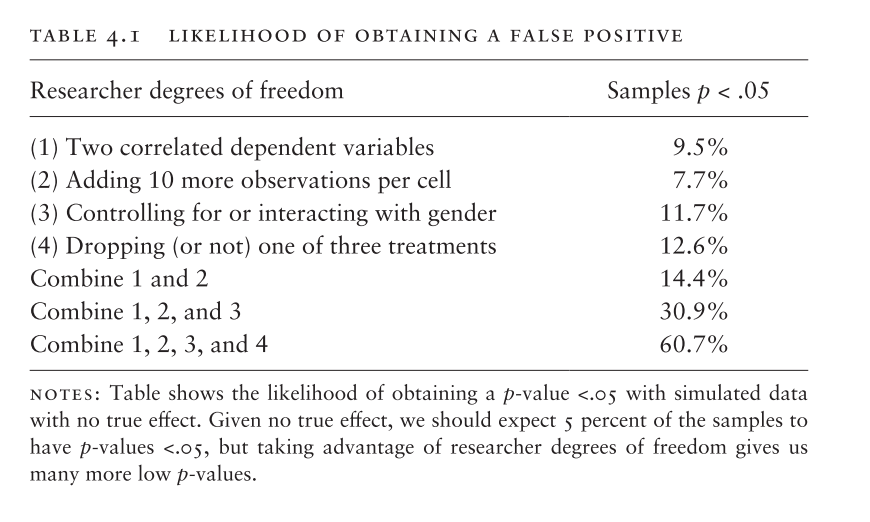
\includegraphics[width=1\linewidth]{docs/images/fp}

\}

\textbackslash caption\{Porcentajes de publicación de acuerdo a significancia de resultados. Imagen de \citet{christensen_Transparent_2019}.\}\label{fig:written}
\textbackslash end\{figure\}

\hypertarget{que-podemos-hacer}{%
\section{¿Que podemos hacer?}\label{que-podemos-hacer}}

Tanto en las ciencias sociales, como en otras disciplinas han ido emergiendo una variedad de recomiendaciones y consejos que contribuyen a la adopción de la transparencia. Por ejemplo, \citet{cruwell_Easy_2018} propone formar investigadores y estudiantes a partir de la promoción de siete principales tópicos: entender la ciencia abierta; acceso abierto; la importancia de los datos, material y código abierto, los análisis reproducibles; los pre-registros; la replicación y, por último, la enseñanza de la ciencia abierta. De forma similar,\ldots{}

\hypertarget{reproducibilidad}{%
\chapter{Reproducibilidad}\label{reproducibilidad}}

En el marco de la denominada ``crisis de la ciencia'', existe una serie de iniciativas que han buscado hacerse cargo de un problema frecuente en las investigaciones, principalmente de caracter cuantitativo. En este sentido, ¿Cuántas veces nos hemos enfrentado a un trabajo publicaco que no comparte sus materiales, y que por tanto, es imposible acceder a los procedimientos que dieron luces de sus resultados?

\hypertarget{herramientas-para-la-transparencia-y-irreproducibilidad}{%
\chapter{Herramientas para la transparencia y irreproducibilidad}\label{herramientas-para-la-transparencia-y-irreproducibilidad}}

\hypertarget{pre-registros}{%
\section{Pre-registros}\label{pre-registros}}

\hypertarget{flujos-de-trabajos-reproducibles.}{%
\section{Flujos de trabajos reproducibles.}\label{flujos-de-trabajos-reproducibles.}}

Otro tratamiento extensivo de la idea de transparencia se da en las TOP Guidelines. Estos son principios que buscan alcanzar un formato de investigación reproducible a tracés del aumento de la transparencia en el proceso y los productos de investigación \citep{nosek_Transparency_2014}. Estos principios sirven de guía a las revistas académicas para poder adherir progresivamente al ideal de transparencia en la ciencia. Son ocho principios:

\begin{enumerate}
\def\labelenumi{\arabic{enumi}.}
\tightlist
\item
  Citación
\item
  Transparencia de datos
\item
  Transparencia de métodos análiticos (código)
\item
  Transparencia de los materiales
\item
  Transparencia del diseño y el análisis
\item
  Preregistro de estudios
\item
  Pre registro de planes de análisis
\item
  Replicación
\end{enumerate}

A grandes rasgos, el principio de citación propone que las normas de citado deben ampliarse también a los datos y códigos, permitiendo reconocer su autoría intelectual \citep{nosek_Promoting_2015}. Los principios de transparencia de datos, métodos análiticos, materiales y diseño y análisis (2 a 5) refieren a la transparencia en su forma más concreta: la apertura del proceso de investigación para su evaluación. El detalle puesto a los principios responde a la generelabizilidad que se le busca dar a los principios. Por ejemplo, un estudio observacional cuantitativo no tiene material que transparentar, pero si datos y métodos análiticos. Asi también, un estudio cualitativo quizás no tenga código que transparentar, pero si un diseño y una bitacora detalla del proceso de análisis. En el caso de los principios relacionados al pre-registro, \citet{nosek_Promoting_2015} argumenta que registrar los estudios los hace más descubribles, incluso si no son públicados. Asi también, los preregistros del plan de análisis contribuyen a distinguir entre los análisis confirmatorios y explotatorios (ver \citet{nosek_preregistration_2018} para un manejo detalado del tema). Por último, el principios de replicación fomenta las oportunidades para la corrección de artículos y redirecciona la investigación en vías más prometedoras \citep{nosek_Promoting_2015}.

Cada uno de estos principios cuenta con tres niveles, que sirven para medir el grado de inclusión de la transparencia por parte de una revista cientifica. La Figura N° \ref{fig:tabtop} muestra cada nivel en relación el principio correspondiente. Se añade un nivel 0 que no cumple los estandares de transparencia con la finalidad de tener una comparación. Por ejemplo, para los estandares de transparencia del método de análisis (código), el nivel 1 dicta que las revistas deben solicitar la existencia del código de análisis, en cambio, el nivel 3 es más estricto en plantear que el código de análisis debe estar almacenado en un repositorio confiable y que el análisis será reproducido durante el proceso de revisión. El mismo método se puede aplicar para la el preregistro del plan de análisis. En el nivel 1 las revistas promueven el uso de preregistros, en cambio, en el nivel 3 los preregistros son obligatorios y también reconocidos. En suma, las TOP Guideliness son una iniciativa que contribuye a la apertura en la ciencia cambiando los requerimientos de las revistas.

Los dos ejemplos entregados (la taxonomía y las TOP Guideliness) perimiten comprender con un poco más de detalle el concepto de transparencia. Sin embargo, aun queda la interrogante del por qué. ¿Cuál es la problemática que lleva a considerar necesaria la adopción de la transparencia? En breve, la respuesta es la crisis en las ciencias, y especificamente en las ciencia sociales.

\begin{figure}

{\centering 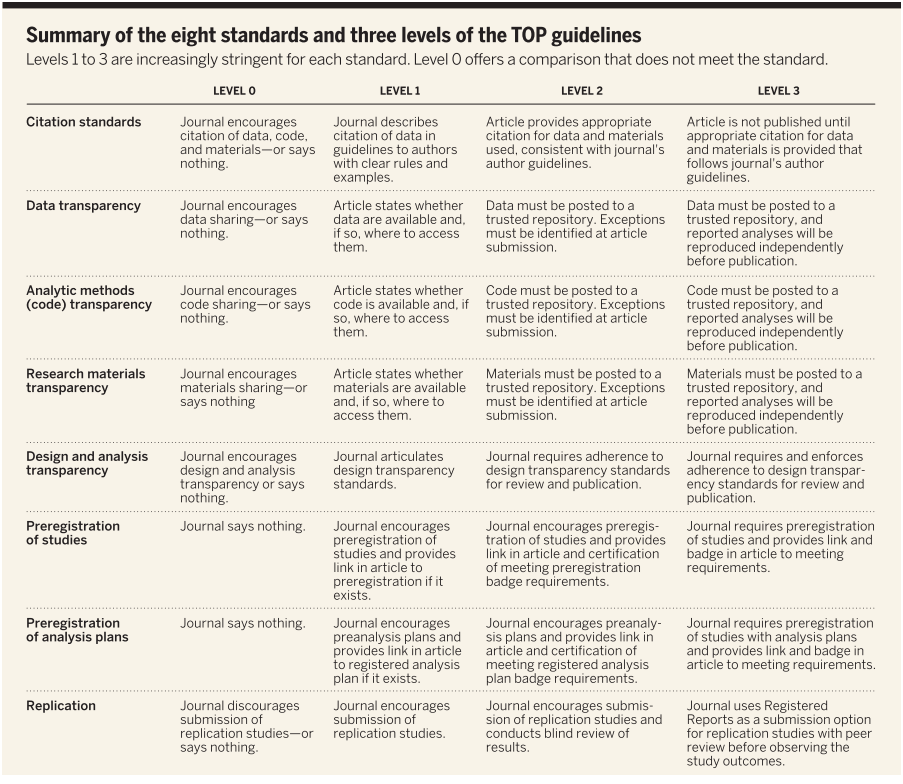
\includegraphics[width=1\linewidth]{docs/images/table_top} 

}

\caption{Variaciones por dimensión de transparencia}\label{fig:tabtop}
\end{figure}

\hypertarget{palabras-finales}{%
\chapter{Palabras finales}\label{palabras-finales}}

Hemos aprendido sobre transparencia y reproducibilidad.

  \bibliography{book.bib,packages.bib}

\end{document}
